\subsection{FFT Field Translations}

From the structure of our kernels of interest (\ref{eq:chpt:2:sec:0:laplace_kernel}), as well as the fact that our equivalent densities and check potentials are arranged on a regular grid (fig. \ref{fig:chpt:2:sec:1:translations}), we notice that the calculation of the downward check potential during $T^{M2L}$ is a convolution,


\begin{flalign}
    \phi = (K \ast q)(x) = \int_{y^{B, d}} K(x-y)q^{A, u}(y)dy
    \label{eq:chpt:3:sec:1:subsec:2:m2l_convolution}
\end{flalign}

When translating the multipole expansion at a box $A$ to a box $B$. From Fourier theory, the property of the Fourier transforms of a convolution is that they are the product of two individual transforms,

\begin{flalign}
    \mathcal{F} \{K \ast q\}(k) = \mathcal{F}\{K\}(k) \cdot \mathcal{F}\{q\}(k)
\end{flalign}

where $k$ denotes the frequencies in Fourier space. We therefore find that the check potential can be computed as,

\begin{flalign}
    \phi(x) = \mathcal{F}^{-1}\{ \mathcal{F}\{K\}(k) \cdot \mathcal{F}\{q\}(k)  \} (x)
\end{flalign}

In practice for the kiFMM the sequence corresponding to $K$ must contain all the unique evaluations of the kernel (\ref{eq:chpt:2:sec:0:laplace_kernel}) between a source box $A$ and a target box $B$. This sequence is constructed with the help of an ancillary data structure known as a `convolution grid'.

We illustrate the construction of the sequences that are required for an FFT based $T^{M2L}$ in $\mathbb{R}^2$, however they are directly applicable to $\mathbb{R}^3$. Consider Figure \ref{fig:chpt:3:sec:1:subsec:2:translations}, which shows a source and target box, each of which is annotated with source equivalent points $y_i$ and target check points, $x_i$, for a $P=2$ expansion.

\begin{figure}
    \centering
    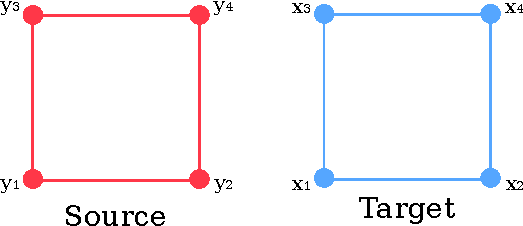
\includegraphics[width=0.6\textwidth]{images/ch_3/m2l_source_target.pdf}
    \caption{A source and target box, with source and target locations on the repsective equivalent and check surface annotated..}
    \label{fig:chpt:3:sec:1:subsec:2:translations}
\end{figure}

The equivalent surface around the source box is \textit{embedded} within a convolution grid, as shown in Figure \ref{fig:chpt:3:sec:1:subsec:2:embed_surface_grid}, such that the number of points on a convolution grid is $P^3$ in $\mathbb{R}^3$ and $P^2$ in $\mathbb{R}^2$ respectively.

\begin{figure}
    \centering
    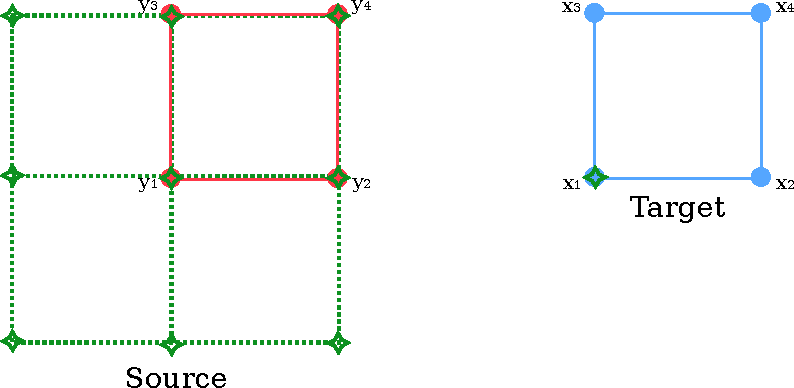
\includegraphics[width=0.6\textwidth]{images/ch_3/embed_surface_grid.pdf}
    \caption{The source equivalent surface is embedded within a (green) convolution grid. The points on the convolution grid are marked with diamonds. An additional diamond is placed on the target check surface, which identifies the point with which kernels are evaluated with respect to.}
    \label{fig:chpt:3:sec:1:subsec:2:embed_surface_grid}
\end{figure}

The unique kernel interactions between the source equivalent surface and the target check surface in (\ref{eq:chpt:3:sec:1:subsec:2:m2l_convolution}) are computed with respect to a single point on the target check surface and the points on the convolution grid. We then see that we must compute the convolution of two sequences in $\mathbb{R}^2$, illustrated in Figure \ref{fig:chpt:3:sec:1:subsec:2:convolution}. Here the first sequence is the unique kernel evaluations taken with respect to a fixed point on the target check surface, and the second sequence is the multipole expansion coefficients mapped to the convolution grid from the source box's equivalent surface. We proceed to take Fourier transforms via the FFT for both of these sequences, and compute their convolution via a Hadamard product.

\begin{figure}
    \centering
    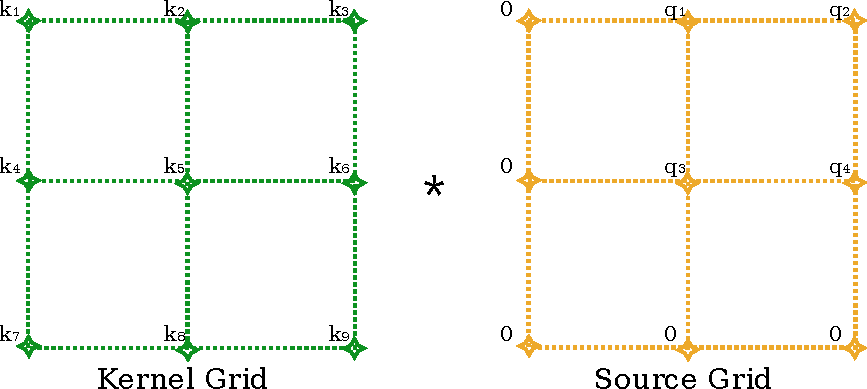
\includegraphics[width=0.6\textwidth]{images/ch_3/convolution.pdf}
    \caption{A Hadamard product is computed between the Fourier transforms sequence of unique kernel evaluations and the multipole expansion coefficients which are also placed on the convolution grid.}
    \label{fig:chpt:3:sec:1:subsec:2:convolution}
\end{figure}

Computing this Hadamard product results in another sequence illustrated in Figure \ref{fig:chpt:3:sec:1:subsec:2:check_potential}, where we have taken care to `flip' the sequence corresponding the unique kernel evaluations as required by the definition of a convolution. We find the final check potentials by taking the inverse Fourier transform of it.

\begin{figure}
    \centering
    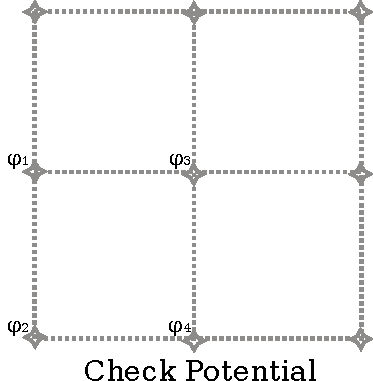
\includegraphics[width=0.3\textwidth]{images/ch_3/check_potential.pdf}
    \caption{The result of the convolution illustrated in Figure \ref{fig:chpt:3:sec:1:subsec:2:convolution}, on the convolution grid. We only identify locations that correspond to check potentials, as the other entries will contain results which are not required, corresponding to redundant computations with this method.}
    \label{fig:chpt:3:sec:1:subsec:2:check_potential}
\end{figure}

We note that although we rely on the existence of a convolution grid to compute the required sequences, in practice we do not compute or store it. We simply require a mapping between the index locations of points on the equivalent surfaces to their corresponding positions on a convolution grid.

Expressed alternatively, we can represent the points on an equivalent surface, $y \in y^{B, u}$, by their respective indices $y_{i, j, k}$ when in $\mathbb{R}^3$. The elements corresponding to the unique kernel interactions are then,

\begin{flalign}
    K_{ijk} = K(x_{000} - y_{ijk})
\end{flalign}

where $x_{000}$ is the index of a point on the target equivalent surface with which the sequence is calculated with respect to. We choose the bottom left corner on the target surface, though in principle any point could be used, it would just amount to a translation of the convolution grid. This results in a 3D sequence $K[ ]$, with elements,

\begin{flalign}
    K[i, j, k] = K_{i, j, k}
\end{flalign}

Again the symmetries of kernels make the Fourier transforms of this quantity something that has the potential to be pre-computed and cached, in a similar way to which the SVD based $T^{M2L}$ could be cached. At runtime, we simply need to look up the corresponding sequence $\hat{K}_t[ ]$ corresponding to a transfer vector $t$ between a given source and target box, and compute the convolution as outlined above. The reduced complexity of the FFT in comparison to an SVD results in greatly faster pre-computation times (see fig. \ref{fig:chpt:3:sec:1:subsec:2:fft_m2l_precomputation} as opposed to fig. \ref{fig:chpt:3:sec:1:subsec:1:svd_m2l_precomputation}).

The Hadamard product has a low computational intensity\footnote{Ratio of flops to memory accesses.}, and naive implementations can be slow in practice regardless of the superior complexity of the FFT based $T^{M2L}$ in comparison to the compressed matrix vector products of the SVD approach outlined in the previous section especially when combined with optimisations to use BLAS3 operations. The authors of the leading multi-node bbFMM \cite{malhotra2015pvfmm} use a strategy of considering sets of siblings together, alongside explicit SIMD to increase the computational intensity of this operation. This approach is re-implemented by the authors of the leading single-node kiFMM \cite{wang2021exafmm}, though involves computes redundant $T^{M2L}$ translations. We explain briefly how this works below, before introducing our own approach which though similar, avoids these redundancies.

Consider a source box alongside its siblings in $\mathbb{R}^3$,

\begin{flalign}
    S = \cup_{i=1}^{N=8} S_i
\end{flalign}

For each unique $T^{M2L}$ we have a sequence $K[ ]$, and can pre-compute a sequence $\hat{K}[ ]$ corresponding to their Fourier transforms. Considering the sibling set $S$'s parent box, we can compute $T^{M2L}$ with respect to the neighbours of $S$'s parent. This results in $64 = 8 \times 8$ for translations between $S$ and the children in a particular neighbour of their parent, with corresponding sequences $\hat{K}[ ]$. We note that not all of these translations are necessarily required, the authors of \cite{malhotra2015pvfmm,wang2021exafmm} simply take the convolutions with respect to zero data used for the corresponding multipole expansion. When repeated for all of the neighbour's of $S$'s parent, we're left with a total of $1664 = 8 \times 8 \times 26$ applications of $T^{M2L}$ for a given sibling set $S$. Despite containing redundant calculations, the implementation is highly cache-optimised. The authors of \cite{malhotra2015pvfmm} proceed by iterating over each of $S$'s parent's neighbours - pulling out the $i^{th}$ frequency component from each - leading to a sequence of length $8 \times 8 \times 26$, they proceed by pulling out the $i^{th}$ frequency component of the Fourier transform of each sibling - leading to a sequence of length 8. The Hadamard product is found by computing 26 individual $8 \times 8$ operation using explicit SIMD. By iterating over $S$'s parent's neighbours in the outer loop the sequence of length $8 \times 8 \times 26$ can be held in memory for each subsequent sibling set.

This strategy is known to perform well. An experiment with the Laplace kernel, order $P=9$ expansions, and 1e6 source/target points takes at most 2.7s to evaluate $T^{M2L}$ on a 6 core Intel i7-9750H processor\footnote{Experiments were repeated 5 times, we report the maximum runtime.}. However, we note that the redundant computations can be reduced.

We begin by noting that for our kernels of interest correspond lead to 316 unique translation vectors $t$ with corresponding $T^{M2L}$ operators, however the majority of these operators correspond to reflections of each other. First introduced by Messner et. al \cite{messner2012optimized} in the context of an SVD based acceleration of $T^{M2L}$, where they attempt to reduce the size of the SVD required for the pre-computation in this approach, one can reduce the number of transfer vectors corresponding to \textit{unique} $T^{M2L}$ to just 16. In the original paper they aimed to demonstrate that with just 16 unique $T^{M2L}$ BLAS3 matrix-matrix products would further reduce the application time of the compressed $T^{M2L}$ operator, however as we demonstrate in Figure \ref{fig:chpt:3:sec:1:subsec:2:blas3}, we don't observe this to have a significant effect on the runtime of the matrix-matrix products of the sizes expected in a typical FMM, at least on modern processors as used during testing.

\begin{figure}
    \centering
    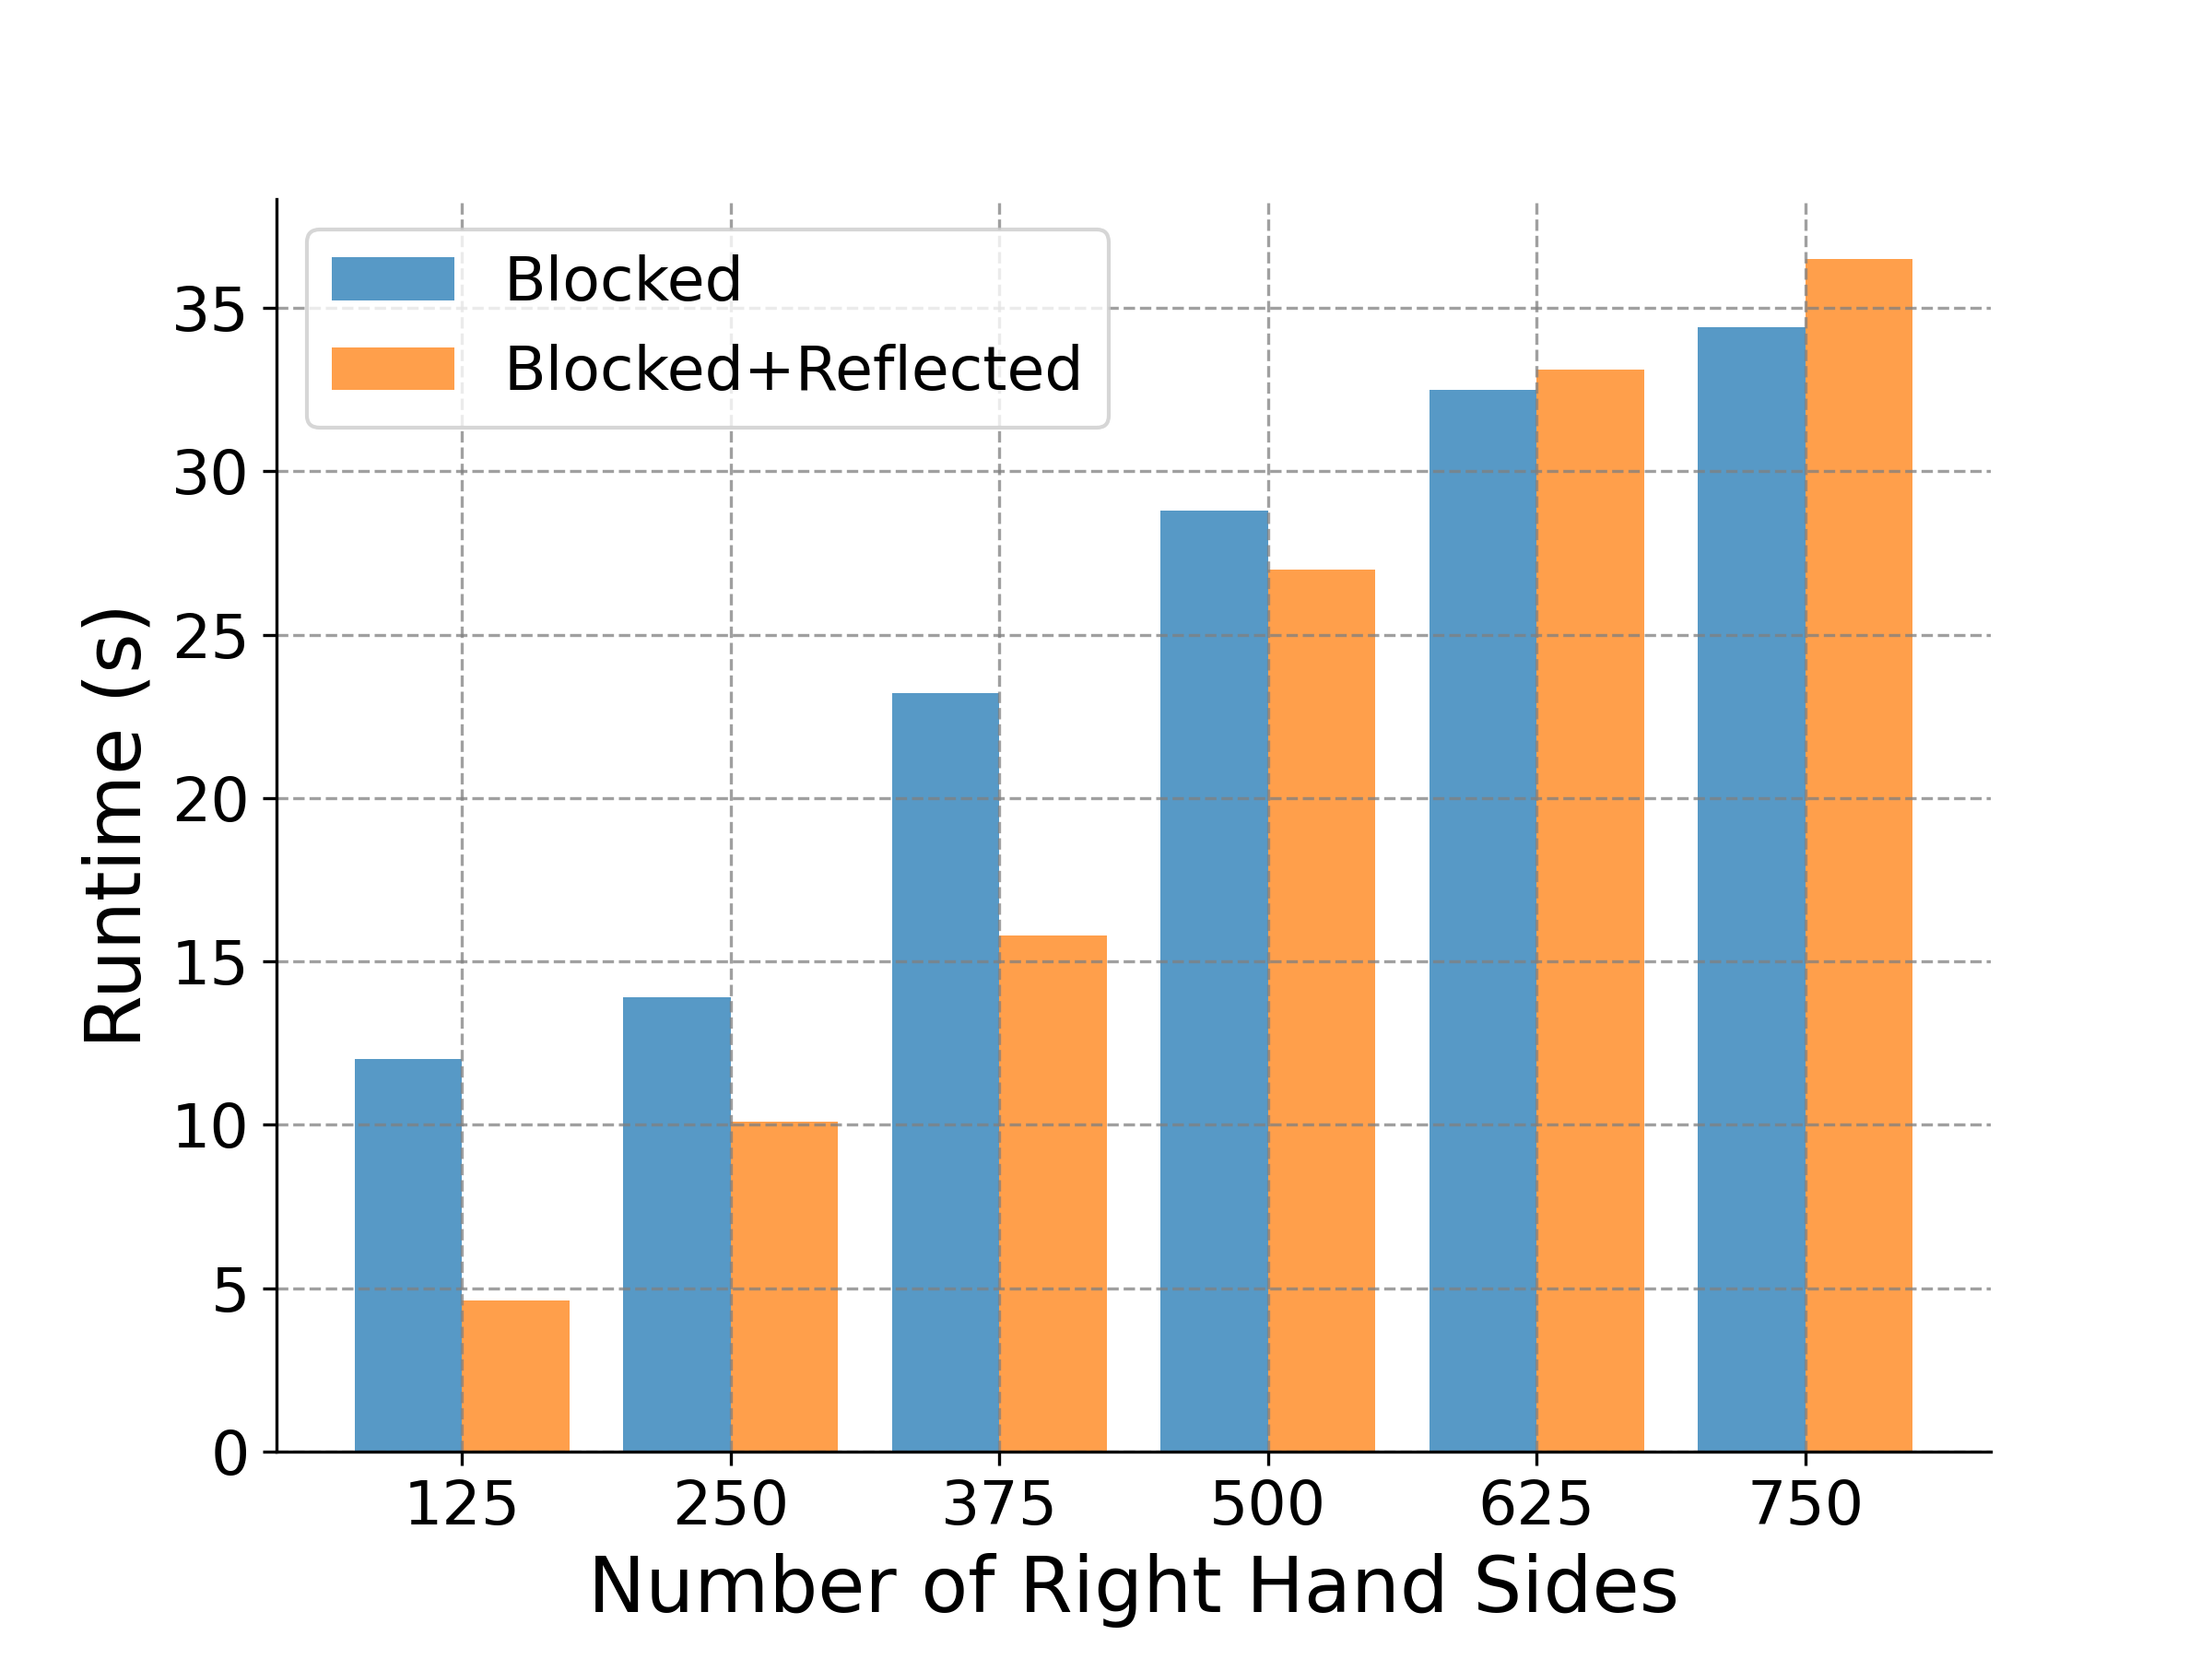
\includegraphics[width=0.6\textwidth]{images/ch_3/blas3.png}
    \caption{In this experiment we compared the runtime for blocking together matrix-matrix products corresponding to $T^{M2L}$ for each of 316 transfer vectors (labelled `Blocked'), to blocking together matrix-matrix products for each of a reduced set of just 16 unique transfer vectors (labelled `Blocked + Reflected'). The left matrix is a random dense matrix generated using double precision floating point numbers, with dimensions matching $T^{M2L}$ for expansion orders of 9, the right matrix is again a random dense matrix generated using double precision floating point numbers chosen to represent the multipole coefficients being translated. To estimate the runtime of application of the blocking approaches, we simply compute the matrix-matrix product with 20 times as many left hand sides ($316/16 = 19.75 \approx 20$) for the reduced blocking scheme, as the blocking scheme doesn't reduce the number of flops in this approach. The matrix-matrix product for the naively blocked scheme is correspondingly computed repeatedly in a loop of length 20, ensuring that both approaches have a matching number of flops. We find that for smaller numbers of left-hand sides, the reducing the set of transfer vectors to make more efficient use of BLAS3 matrix-matrix products does help significantly, however for larger numbers of left-hand sides greater than approximately 500, which is typical for the FMM, there is little difference with this optimisation. Experiments are taken on a 6 core Intel i7-9750 processor using Open BLAS, we report maximum runtimes over 5 runs for each set of parameters.}
    \label{fig:chpt:3:sec:1:subsec:2:blas3}
\end{figure}

In order to see how we arrive at 16 unique $T^{M2L}$ operators we introduce two symmetries, building upon the discussion in \cite{messner2012optimized}. They describe two planes of symmetry, axial and diagonal, when considering a source box $A$ and a target box $B$ during a given interaction specified by a $T^{M2L}$ operator. This is sketched for $\mathbb{R}^2$ for clarity in Figure \ref{fig:chpt:3:sec:1:subsec:2:symmetries}, where we show three sources $A$ with their respective transfer vectors, $t$, with respect to $B$. These boxes describe the equivalent/check surfaces described above for the kiFMM and the quadrature points are labelled by an index coordinate for an expansion of $P=2$. The axial planes of symmetry are given by $t_1 = 0$, $t_2 = 0$ and $t_3 = 0$ in $\mathbb{R}^3$, each dividing $\mathbb{R}^3$ into two parts centered on the target box $B$. Combining all three plane divides $\mathbb{R}^3$ into octants centered on $B$, we refer to $\mathbb{R}^3_+$ as the \textit{reference octant}. The diagonal planes of symmetry are given by $t_1 = t_2$, $t_1 = t_3$ and $t_2 = t_3$ in $\mathbb{R}^3$. We restrict ourselves to diagonal symmetries that lie in the reference octant. Combining the axial and diagonal symmetries we obtain a \textit{reference cone},

\begin{flalign}
    \mathbb{R}^3_{\text{sym}} = \{ \mathbb{R}^3_{\text{sym}} \subset \mathbb{R}^3 : t_1 \geq t_2 \geq t_3 \text{ with } t \in \mathbb{R}^3 \}
    \label{eq:chpt:3:sec:1:subsec:2:reference_cone}
\end{flalign}

We identify a subset of transfer vectors $T_{\text{sym}} = T \cap  \mathbb{R}^3_{\text{sym}}$ from which all transfer vectors for $B$ can be expressed as reflections around the axes of symmetry. Explicitly to find $t$ within $T_{\text{sym}}$, we apply the following rule

\begin{enumerate}
    \item A \textit{axial symmetry} given by say $t_1 = 0$ as shown in Figure \ref{fig:chpt:3:sec:1:subsec:2:symmetries}, we invert the corresponding component of the index coordinate
    \[
        \alpha \leftarrow (P-(\alpha_1-1), \alpha_2, \alpha_3) \text{ and } \beta \leftarrow (P-(\beta_1-1), \beta_2, \beta_3)
    \]
    \item A \textit{diagonal symmetry} given by say $t_1 = t_2$, w swap the corresponding components of the index coordinate as,
    \[
        \alpha \leftarrow (\alpha_2, \alpha_1, \alpha_3) \text{ and } \beta \leftarrow (\beta_2, \beta_1, \beta_3)
    \]
\end{enumerate}


Where as before $P$ stands for expansion order. When these rules are applied to the 316 unique transfer vectors for our kernels of interest, we find that $|T_{\text{sym}}|  = 16$.

\begin{figure}
    \centering
    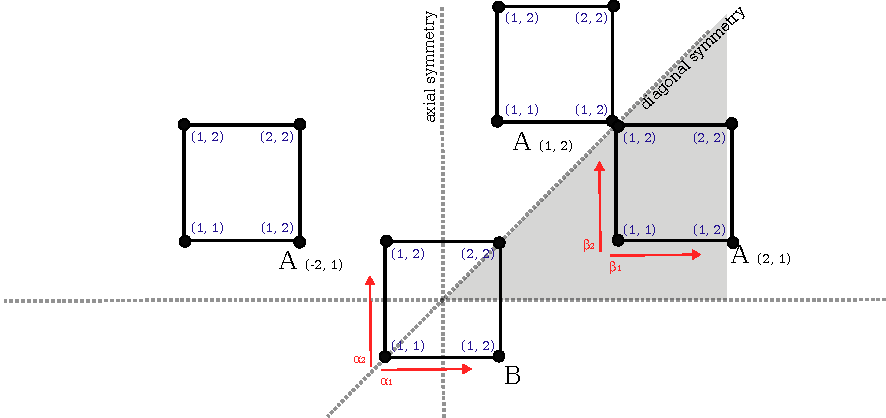
\includegraphics[width=\textwidth]{images/ch_3/symmetries.pdf}
    \caption{Here we show the axial and diagonal symmetries of three source boxes labelled $A$ with respect to a target box $B$ in $\mathbb{R}^2$ for expansion order $P=2$. The quadrature points are labelled with index coordinates taken with respect to the lower left corner of the box. The only transfer vector here the constraints of being in the `reference cone', which is shaded in grey, is $t=(2, 1)$ and therefore corresponds to the only $T^{M2L}$ that needs to be pre-computed. This figure is adapted from \cite{messner2012optimized} for the kiFMM as opposed to the bbFMM as originally presented.}
    \label{fig:chpt:3:sec:1:subsec:2:symmetries}
\end{figure}

Utilising this redundancy for the FFT accelerated $T^{M2L}$ means that one only has to precompute Fourier transform of Kernel sequences $K[]$ corresponding to transfer vectors in $T_{\textit{sym}}$. In order to reduce the number of flops required for computing $T^{M2L}$ during the algorithm we notice that $T^{M2L}$ is calculated for a box $B$ from a halo consisting of its interaction list, i.e. the children of $B$'s parent which it does not lie adjacent to. There is a conjugacy in this relationship meaning that if $A$ is in that set of boxes for $B$, then $B$ is correspondingly in that set of boxes for $A$. This means that we can `invert' the application of the $T^{M2L}$ operator. Instead of attempting to compute the check potential at $B$ from boxes $A$ in its halo, we can instead compute the convolutions corresponding to just 16 unique $T^{M2L}$ for the multipole coefficients at $B$ and scatter the resulting check potential to their corresponding boxes in $B$'s halo. This means that we are only computing 16 convolution operations with respect to each box, in comparison the 1664 as in previous implementations.

This transforms the problem into one that is bound by memory accesses. To alleviate this we take a similar approach to the state of the art softwares mentioned above, and consider sibling sets $S$ at a time. We iterate over sibling sets in parallel, pulling in references to $S$'s parent's neighbours' children into memory in each parallel thread. These constitute all the scatter locations for the check potentials computed for each box in $S$. By doing this however we reduce the number of cache-misses during the scatter operation as we an save all the corresponding check potentials to a box in $S$'s halo at once. For the same benchmark problem above we reported for the state of the art approach of \cite{malhotra2015pvfmm}, we compute $T^{M2L}$ in 6.8s \footnote{Experiments were repeated 5 times, we report the maximum runtime.}.

The effect of memory ordering and access on runtimes is clear, and significant, for this operation. As of writing are still working on an optimal memory ordering in the implementation of this approach, which if we are able to find would constitute a new algorithm for sparsifying $T^{M2L}$ via the FFT for algebraic FMMs discretised on regular grids, as the number flops in our approach is greatly reduced.

\begin{figure}
    \centering
    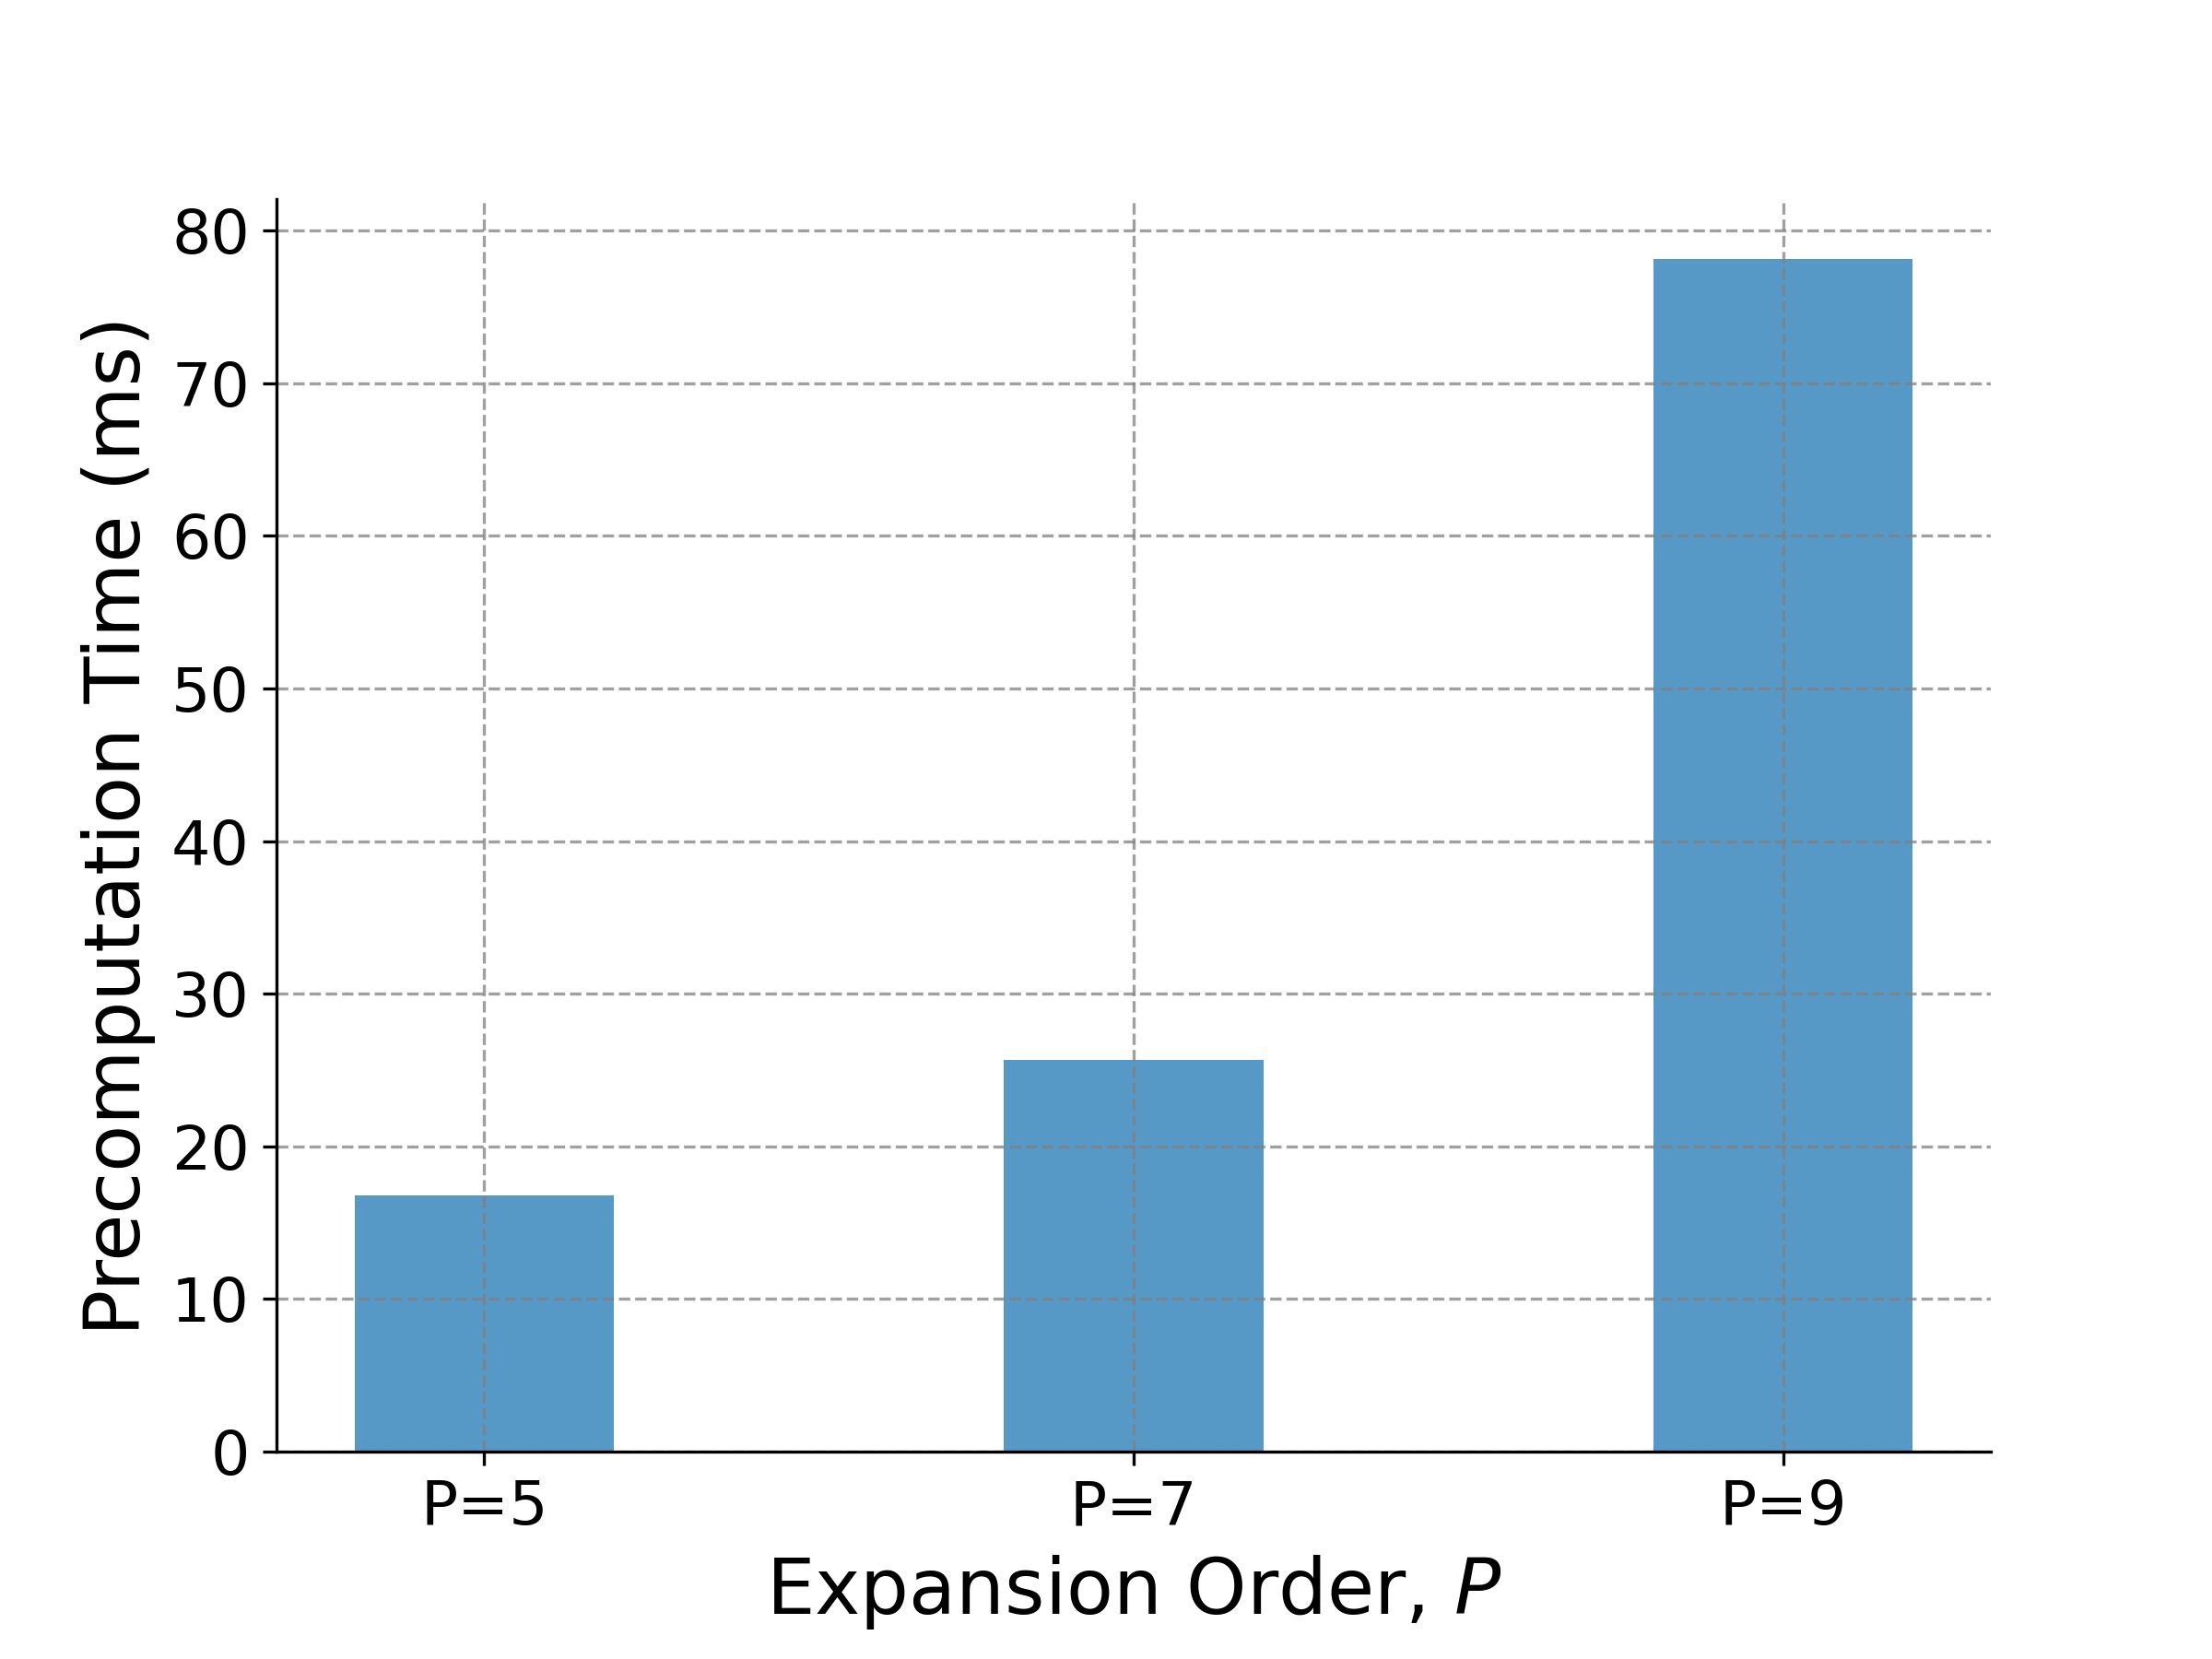
\includegraphics[width=0.6\textwidth]{images/ch_3/fft_m2l_precomputation.png}
    \caption{Here we illustrate the precomputation time to compute the FFTs required of $T^{M2L}$ for a selection of expansion orders for all 316 unique transfer vectors for the Laplace kernel. We highlight the approximately 500x runtime advantage over the precomputations required for the SVD implementation (fig. \ref{fig:chpt:3:sec:1:subsec:1:svd_m2l_precomputation}). Experiments are taken on a 6 core Intel i7-9750 processor using Open BLAS, we report maximum runtimes over 5 runs
    for each set of parameters.}
    \label{fig:chpt:3:sec:1:subsec:2:fft_m2l_precomputation}
\end{figure}